\documentclass[11pt,a4paper]{article}

\usepackage[margin=1.8cm]{geometry}
\usepackage{microtype}
\usepackage{amsmath}
\usepackage{booktabs}
\usepackage{longtable}
\usepackage{array}
\usepackage{hyperref}
\usepackage{tikz}

\usetikzlibrary{arrows.meta, positioning, shapes.geometric, calc}

\hypersetup{
  colorlinks=true,
  linkcolor=blue!50!black,
  urlcolor=teal!50!black
}

\setlength{\parindent}{0pt}
\setlength{\parskip}{6pt}
\renewcommand{\arraystretch}{1.2}

\definecolor{ink}{HTML}{213547}
\definecolor{softblue}{HTML}{DCEAF7}
\definecolor{softgreen}{HTML}{DFF4E5}
\definecolor{softorange}{HTML}{F8EAD7}
\definecolor{softrose}{HTML}{F7DBE6}
\definecolor{softgold}{HTML}{F8F2CF}

\newcommand{\studybox}[2]{%
  \par\medskip
  \noindent\fcolorbox{ink}{white}{%
    \parbox{0.96\linewidth}{\textbf{#1}\par #2}%
  }%
  \par\medskip
}

\begin{document}

\begin{titlepage}
\centering
{\Large \textbf{Retrieval Engine Competition Project}}\\[0.6cm]
{\large Cleaned structure, study workbook, and report}\\[1.2cm]

\studybox{Project Goal}{Build a retrieval pipeline for the Kaggle competition, keep the code runnable, and turn the repository into a better study object by consolidating scattered notebooks into one workbook and one A4 report.}

\vspace{0.6cm}

\begin{tabular}{>{\bfseries}p{0.28\linewidth} p{0.58\linewidth}}
Project & Retrieval engine competition pipeline \\
Main code & \texttt{src/} + \texttt{main.py} \\
Workbook & \texttt{notebooks/retrieval\_project\_workbook.ipynb} \\
Report & \texttt{report/retrieval\_project\_report.pdf} \\
Date & March 11, 2026 \\
\end{tabular}

\vfill

{\small This PDF is designed as a memorable study guide: it uses diagrams, shapes, compact summaries, and an appendix with guided practice.}
\end{titlepage}

\tableofcontents
\newpage

\section{Project At A Glance}

The cleaned repository now separates execution, learning, and reporting:

\begin{itemize}
\item \texttt{src/} contains the runnable retrieval system.
\item \texttt{notebooks/retrieval\_project\_workbook.ipynb} is the single teaching-first notebook.
\item \texttt{report/retrieval\_project\_report.pdf} is the formal A4 summary with appendix material.
\end{itemize}

\studybox{What Was Removed}{The old notebook collection had overlapping responsibilities: data exploration, explanation, Kaggle submission, model intuition, and reporting were split across several files. Those were merged into one workbook so the learning path is linear instead of fragmented.}

\subsection{Clean Repository Layout}

\begin{tabular}{p{0.29\linewidth} p{0.63\linewidth}}
\toprule
\textbf{Path} & \textbf{Purpose} \\
\midrule
\texttt{src/config.py} & Central runtime settings for evaluation and submission generation. \\
\texttt{src/preprocess.py} & Builds the shared \texttt{content} field for documents and queries. \\
\texttt{src/models.py} & TF-IDF, BM25+, dense retrieval, and hybrid reranking. \\
\texttt{src/evaluation.py} & Precision@K, Recall@K, MRR, and MAP. \\
\texttt{src/utils.py} & Data loading, CSV writing, and submission validation. \\
\texttt{src/pipeline.py} & End-to-end orchestration with clearer helper functions. \\
\texttt{notebooks/retrieval\_project\_workbook.ipynb} & One visual workbook with plots, diagrams, exercises, and code explanations. \\
\texttt{report/retrieval\_project\_report.tex} & LaTeX source for this A4 report. \\
\bottomrule
\end{tabular}

\section{Dataset Snapshot}

The local data used in this project contains:

\begin{itemize}
\item 216{,}041 documents,
\item 327 training queries,
\item 141 test queries,
\item 327 qrels entries for evaluation.
\end{itemize}

The document categories are strongly imbalanced, which matters because retrieval behavior often changes by domain vocabulary.

\begin{center}
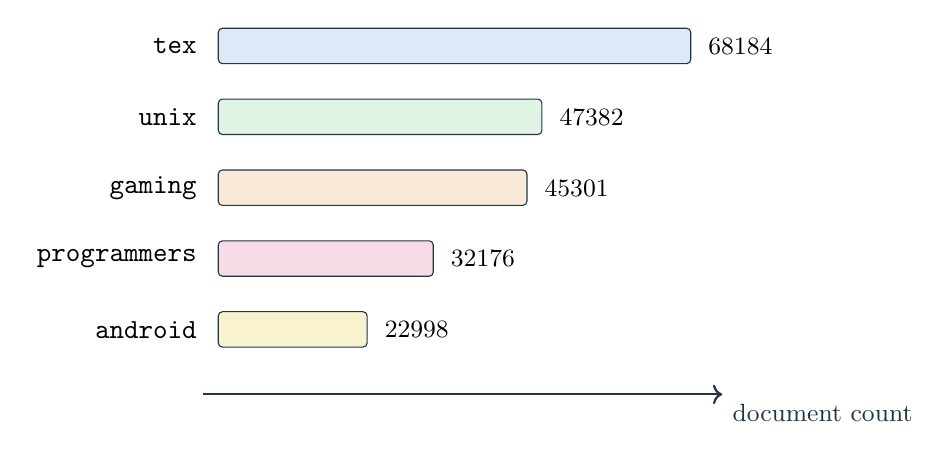
\begin{tikzpicture}[x=1cm,y=1cm]
\draw[->, thick, color=ink] (0,0.6) -- (6.6,0.6) node[below right] {\small document count};
\filldraw[fill=softblue, draw=ink, rounded corners=1.5pt] (0.2,4.8) rectangle (6.20,5.25);
\node[anchor=east] at (0.05,5.02) {\texttt{tex}};
\node[anchor=west] at (6.30,5.02) {\small 68184};

\filldraw[fill=softgreen, draw=ink, rounded corners=1.5pt] (0.2,3.9) rectangle (4.31,4.35);
\node[anchor=east] at (0.05,4.12) {\texttt{unix}};
\node[anchor=west] at (4.41,4.12) {\small 47382};

\filldraw[fill=softorange, draw=ink, rounded corners=1.5pt] (0.2,3.0) rectangle (4.12,3.45);
\node[anchor=east] at (0.05,3.22) {\texttt{gaming}};
\node[anchor=west] at (4.22,3.22) {\small 45301};

\filldraw[fill=softrose, draw=ink, rounded corners=1.5pt] (0.2,2.1) rectangle (2.93,2.55);
\node[anchor=east] at (0.05,2.32) {\texttt{programmers}};
\node[anchor=west] at (3.03,2.32) {\small 32176};

\filldraw[fill=softgold, draw=ink, rounded corners=1.5pt] (0.2,1.2) rectangle (2.09,1.65);
\node[anchor=east] at (0.05,1.42) {\texttt{android}};
\node[anchor=west] at (2.19,1.42) {\small 22998};
\end{tikzpicture}
\end{center}

\studybox{Small But Important Observation}{The dataset contains one empty document body. This is a good reminder that retrieval systems are not only ranking systems; they are also data-cleaning systems.}

\section{Steps We Took}

\begin{enumerate}
\item \textbf{Inspected the raw JSON files.} We identified the shared fields used across documents and queries: title, text, tags, and category.
\item \textbf{Normalized the text path.} We created one common \texttt{content} field so all models compare like with like.
\item \textbf{Implemented multiple retrieval strategies.} The project supports TF-IDF, BM25+, dense retrieval, and a lexical-plus-semantic hybrid.
\item \textbf{Evaluated with ranked-retrieval metrics.} We measured Precision@K, Recall@K, MRR, and MAP on the training split.
\item \textbf{Generated Kaggle-ready files.} The pipeline writes per-model CSV files and validates the final submission against the sample template.
\item \textbf{Cleaned the repository for learning.} We replaced the notebook sprawl with one workbook and one report.
\end{enumerate}

\begin{center}
\resizebox{\linewidth}{!}{%
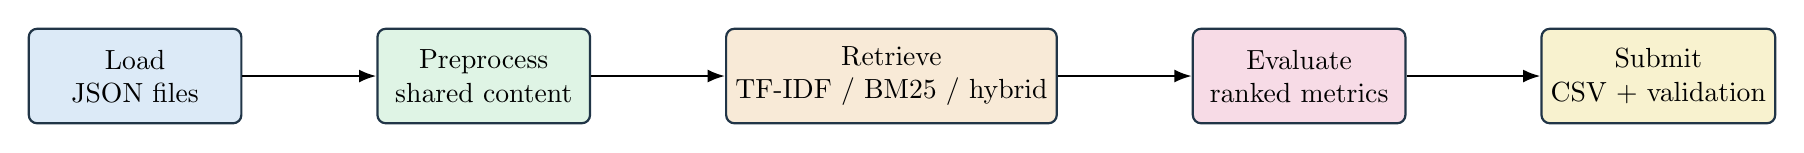
\begin{tikzpicture}[
  node distance=1.7cm,
  box/.style={draw=ink, rectangle, rounded corners=3pt, minimum width=2.7cm, minimum height=1.2cm, align=center, thick},
  >={Latex[length=2.2mm]}
]
\node[box, fill=softblue] (load) {Load\\JSON files};
\node[box, fill=softgreen, right=of load] (prep) {Preprocess\\shared content};
\node[box, fill=softorange, right=of prep] (rank) {Retrieve\\TF-IDF / BM25 / hybrid};
\node[box, fill=softrose, right=of rank] (eval) {Evaluate\\ranked metrics};
\node[box, fill=softgold, right=of eval] (submit) {Submit\\CSV + validation};

\draw[->, thick] (load) -- (prep);
\draw[->, thick] (prep) -- (rank);
\draw[->, thick] (rank) -- (eval);
\draw[->, thick] (eval) -- (submit);
\end{tikzpicture}
}
\end{center}

\section{Modeling Choices}

\subsection{TF-IDF}

TF-IDF is a strong lexical baseline because it rewards terms that are frequent in a document but not frequent everywhere in the corpus. In this project, it uses unigram and bigram features and cosine similarity.

\subsection{BM25+}

BM25+ is another lexical ranker, but its scoring curve differs from TF-IDF. It usually handles term frequency saturation and document length normalization more explicitly, which can change the top-ranked items even when both models use the same input text.

\subsection{Hybrid Semantic Reranking}

The hybrid model works in two layers:

\begin{center}
\resizebox{\linewidth}{!}{%
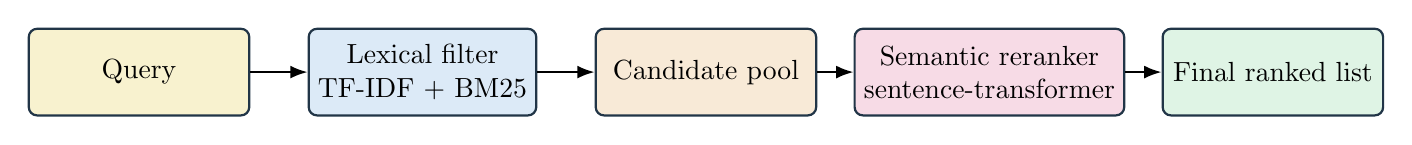
\begin{tikzpicture}[
  box/.style={draw=ink, rectangle, rounded corners=3pt, minimum width=2.8cm, minimum height=1.1cm, align=center, thick},
  >={Latex[length=2.2mm]}
]
\node[box, fill=softgold] (query) at (0,0) {Query};
\node[box, fill=softblue] (lexical) at (3.6,0) {Lexical filter\\TF-IDF + BM25};
\node[box, fill=softorange] (pool) at (7.2,0) {Candidate pool};
\node[box, fill=softrose] (semantic) at (10.8,0) {Semantic reranker\\sentence-transformer};
\node[box, fill=softgreen] (final) at (14.4,0) {Final ranked list};

\draw[->, thick] (query) -- (lexical);
\draw[->, thick] (lexical) -- (pool);
\draw[->, thick] (pool) -- (semantic);
\draw[->, thick] (semantic) -- (final);
\end{tikzpicture}
}
\end{center}

This is a useful design because a cheap lexical stage keeps recall high, while the semantic stage can repair some vocabulary mismatch errors.

\studybox{Memorable Mental Model}{Think of the hybrid system as a two-stage interview process. TF-IDF and BM25 decide who gets invited into the room. The semantic reranker decides who should sit at the front of the table.}

\subsection{Fast Study Benchmark}

Inside the workbook, we run a smaller experiment on a \texttt{tex} subset with 30{,}000 documents and 12 queries so the student can iterate quickly.

\begin{tabular}{lrrrr}
\toprule
\textbf{Model} & \textbf{Precision@10} & \textbf{Recall@10} & \textbf{MRR@10} & \textbf{MAP@10} \\
\midrule
TF-IDF & 0.0750 & 0.3639 & 0.1605 & 0.1159 \\
BM25+ & 0.0500 & 0.2042 & 0.3417 & 0.1646 \\
\bottomrule
\end{tabular}

These values are not presented as the final competition result. They are a teaching benchmark designed to make metric tradeoffs visible quickly.

\section{Submission Workflow}

The project generates:

\begin{itemize}
\item one CSV per configured model,
\item one final upload file based on the chosen \texttt{final\_model},
\item a validation check against the sample submission template.
\end{itemize}

Centralizing runtime settings in \texttt{src/config.py} makes the pipeline easier to explain and safer to modify. Instead of hunting through \texttt{src/pipeline.py} for scattered constants, the user now has one place to adjust the main switches.

\section{How To Study The Project}

Recommended order:

\begin{enumerate}
\item Open the workbook and run the data summary cell.
\item Study the category and length plots before reading the models.
\item Run the pipeline diagram cell and explain it aloud from memory.
\item Use the toy example to predict the ranking before executing the code.
\item Run the fast benchmark and compare TF-IDF against BM25+.
\item Read the appendix and complete at least two active-learning exercises.
\end{enumerate}

\appendix

\section{Appendix: Complete Explanations}

\subsection{Why The Shared \texttt{content} Field Matters}

The data files contain several text sources. Documents have title, body text, and tags. Queries have title and text. If different models read different text combinations, then model comparisons stop being fair. The project avoids that problem by building one normalized \texttt{content} field for every item. Lowercasing is also done centrally so lexical models behave consistently.

\subsection{Metric Formulas}

\[
\text{Precision@K} = \frac{\text{relevant items in top K}}{K}
\]

\[
\text{Recall@K} = \frac{\text{relevant items in top K}}{\text{all relevant items}}
\]

\[
\text{MRR@K} = \frac{1}{|Q|} \sum_{q \in Q} \frac{1}{\text{rank of first relevant result for } q}
\]

\[
\text{AP@K} = \frac{1}{|R_q|} \sum_{k=1}^{K} \text{Precision@k} \cdot \mathbf{1}[\text{item at } k \text{ is relevant}]
\]

MAP is the mean of AP over queries.

\subsection{Code Walkthrough}

\begin{longtable}{p{0.22\linewidth} p{0.72\linewidth}}
\toprule
\textbf{File} & \textbf{Explanation} \\
\midrule
\endhead
\texttt{src/config.py} & Stores evaluation and submission settings in one dataclass so the pipeline is easier to configure and explain. \\
\texttt{src/preprocess.py} & Converts mixed cell values to text, joins selected fields, lowercases them, and guarantees a shared \texttt{content} representation. \\
\texttt{src/models.py} & Implements four retrieval paths. TF-IDF uses sparse lexical vectors, BM25+ uses token-based probabilistic ranking, dense retrieval encodes text into embeddings, and the hybrid path reranks lexical candidates semantically. \\
\texttt{src/evaluation.py} & Calculates retrieval metrics query by query, skipping queries without ground-truth relevance labels. \\
\texttt{src/utils.py} & Reads JSON data, converts qrels into a lookup map, writes Kaggle CSV files in the correct row order, and validates submission format. \\
\texttt{src/pipeline.py} & Splits the full workflow into preparation, evaluation, and submission-generation helpers so the code reads as a sequence of project steps instead of one large function. \\
\texttt{main.py} & Keeps the command-line entrypoint minimal by delegating work to the pipeline module. \\
\bottomrule
\end{longtable}

\subsection{Practices And Active Learning Exercises}

\studybox{Exercise 1: Preprocessing Sensitivity}{Remove \texttt{tags} from the document \texttt{content} field and rerun the workbook benchmark. Write down which queries changed most and why.}

\studybox{Exercise 2: Metric Tradeoffs}{Change \texttt{top\_k} from 10 to 5. Predict which metric should increase and which one may decrease before you run the code.}

\studybox{Exercise 3: Domain Shift}{Repeat the fast study benchmark in another category such as \texttt{android} or \texttt{unix}. Compare whether the same model still wins on the same metric.}

\studybox{Exercise 4: Error Analysis}{Pick one query where TF-IDF and BM25+ disagree. Inspect the titles of the top five retrieved documents and classify the error: vocabulary mismatch, noisy text, missing context, or data issue.}

\studybox{Exercise 5: Hybrid Reasoning}{Without running the hybrid model, identify two queries that would probably benefit from semantic reranking. Explain what lexical retrieval is likely to miss.}

\studybox{Exercise 6: Code Reading}{Read \texttt{run\_tfidf\_search}, \texttt{run\_bm25\_search}, and \texttt{evaluate\_retrieval}. Then explain the pipeline aloud in five sentences without opening the files again.}

\subsection{Practical Study Advice}

\begin{itemize}
\item Always connect a metric change to a ranking change on at least one real query.
\item Use the pipeline diagram until you can redraw it from memory.
\item Treat the workbook as the interactive lab and this PDF as the compact revision sheet.
\item Do not jump to the hybrid model before you can explain lexical retrieval clearly.
\end{itemize}

\end{document}
